\documentclass{standalone}

\usepackage{pgfplots}
\pgfplotsset{compat=1.10}   % in my packages used compat=1.15
\usepgfplotslibrary{fillbetween}
\usepackage{pgf}
\usepackage{tikz}
\usetikzlibrary{patterns,arrows,calc,decorations.pathmorphing,backgrounds, positioning,fit,petri,decorations.fractals}
\usetikzlibrary{matrix}

\usepackage[table,dvipsnames]{tudscrcolor}

\usepackage[default]{opensans}

\begin{document}
	\color{cddarkblue}
	
	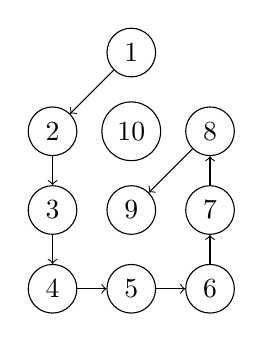
\begin{tikzpicture}
	% Knoten
		\node (1) at (1,0)  [circle,draw] {1};
		\node (2) at (0,-1) [circle,draw] {2};
		\node (3) at (0,-2) [circle,draw] {3};
		\node (4) at (0,-3) [circle,draw] {4};
		\node (5) at (1,-3) [circle,draw] {5};
		\node (6) at (2,-3) [circle,draw] {6};
		\node (7) at (2,-2) [circle,draw] {7};
		\node (8) at (2,-1) [circle,draw] {8};
		\node (9) at (1,-2) [circle,draw] {9};
		\node (10) at (1,-1) [circle,draw] {10};
	% Kanten
		\draw[->] (1) to (2);
		\draw[->] (2) to (3);
		\draw[->] (3) to (4);
		\draw[->] (4) to (5);
		\draw[->] (5) to (6);
		\draw[->] (6) to (7);
		\draw[->] (7) to (8);
		\draw[->] (8) to (9);
	\end{tikzpicture}
	
	\hspace{2em}
	
	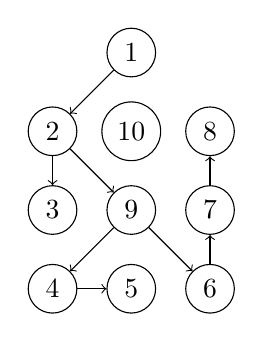
\begin{tikzpicture}
	% Knoten
		\node (1) at (1,0)  [circle,draw] {1};
		\node (2) at (0,-1) [circle,draw] {2};
		\node (3) at (0,-2) [circle,draw] {3};
		\node (4) at (0,-3) [circle,draw] {4};
		\node (5) at (1,-3) [circle,draw] {5};
		\node (6) at (2,-3) [circle,draw] {6};
		\node (7) at (2,-2) [circle,draw] {7};
		\node (8) at (2,-1) [circle,draw] {8};
		\node (9) at (1,-2) [circle,draw] {9};
		\node (10) at (1,-1) [circle,draw] {10};
	% Kanten
		\draw[->] (1) to (2);
		\draw[->] (2) to (3);
		\draw[->] (2) to (9);
		\draw[->] (9) to (4);
		\draw[->] (4) to (5);
		\draw[->] (9) to (6);
		\draw[->] (6) to (7);
		\draw[->] (7) to (8);
	\end{tikzpicture}
	
	\hspace{2em}
	
	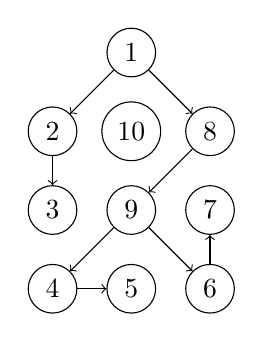
\begin{tikzpicture}
	% Knoten
		\node (1) at (1,0)  [circle,draw] {1};
		\node (2) at (0,-1) [circle,draw] {2};
		\node (3) at (0,-2) [circle,draw] {3};
		\node (4) at (0,-3) [circle,draw] {4};
		\node (5) at (1,-3) [circle,draw] {5};
		\node (6) at (2,-3) [circle,draw] {6};
		\node (7) at (2,-2) [circle,draw] {7};
		\node (8) at (2,-1) [circle,draw] {8};
		\node (9) at (1,-2) [circle,draw] {9};
		\node (10) at (1,-1) [circle,draw] {10};
	% Kanten
		\draw[->] (1) to (2);
		\draw[->] (2) to (3);
		\draw[->] (1) to (8);
		\draw[->] (8) to (9);
		\draw[->] (9) to (4);
		\draw[->] (9) to (6);
		\draw[->] (4) to (5);
		\draw[->] (6) to (7);
	\end{tikzpicture}
\end{document}